\documentclass[12pt,a4paper]{report}
\usepackage[utf8]{inputenc}
\usepackage[german]{babel}
\usepackage[T1]{fontenc}
\usepackage{amsmath}
\usepackage{amsfonts}
\usepackage{amssymb}
\usepackage{graphicx}
\usepackage{titlesec} 
\titleformat{\chapter}{\bfseries\huge}{\thechapter.\quad}{0ex}{\vspace{0.1ex}}
[\vspace{0.1ex}]%\rule{\textwidth}{0.3pt}]
\author{Fabio Greco - Franziska Theis}

\title{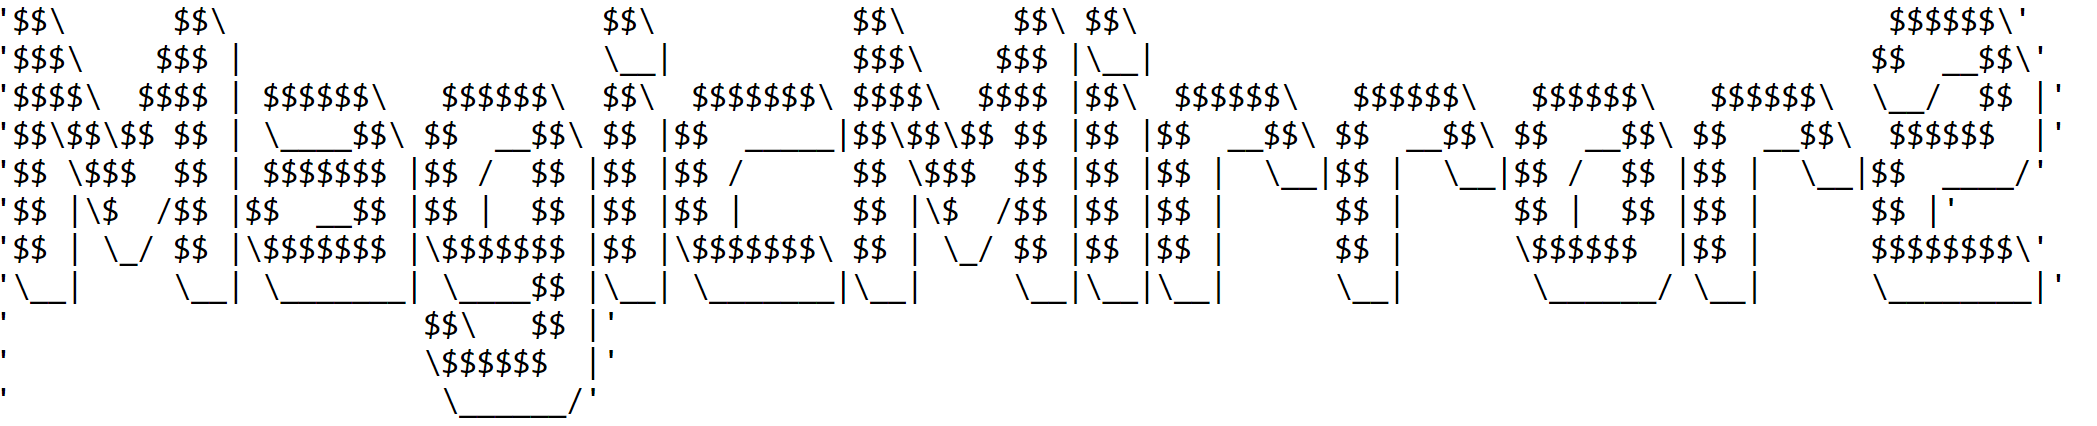
\includegraphics[scale=1]{Cover.png} \\
Implementierung eines personalisierten intelligenten Spiegels (Magic Mirror) 
}

\begin{document}
%\hspace{-50pt}
\maketitle

\chapter{Hinführung}
In Zeiten von Digitalisierung und einem ständigem Online-sein setzt das Projekt in diesem Alltag an. Ein Spiegel, der bisher nur dem Zweck diente, sich selbst darin zu sehen, wird nun erweitert. Er soll den Benutzer mit Nachrichten aus der Welt informieren, mit aktuellem Wetter auf den Tag vorbereiten und die bevorstehenden Termine bereits beim Zähneputzen anzeigen. Kurzum, der Magic Mirror, oder auch Smart Mirror genannt, soll ein Alleskönner werden. 
\section{Problemstellung}
Der Magic Mirror ist eine weitverbreitete Anwendung des Raspberry Pis, weswegen bereits mehrere Betriebssysteme verfügbar sind. Die Betriebssysteme werden später vorgestellt. 
Die Auswahl und Konfigurierung der zugehörigen Module, beispielsweise ein Kalender oder ein Newsfeed, werden ebenfalls in den weiteren Kapiteln beschrieben. 
Damit der Magic Mirror für mehrere Personen nutzbar wird, welche verschiedene Interessen haben und somit andere Module als wichtig empfinden, soll eine Personalisierung implementiert werden. Wie zwischen den Profilen gewechselt werden soll, ist nicht vorgegeben, weshalb auch hier im Laufe des Berichts mehrere Möglichkeiten evaluiert werden. 
Der Controller des Magic Mirror ist der Raspberry Pi. Bei der Ausarbeitung des Projekts sind daher einige Vorkenntnisse, sowie ein Verständnis über das Betriebssystems des Raspberry Pis unabdingbar. Deshalb wird dazu im nächsten Kapitel eine kurze Einführung gegeben.



\chapter{Ziele für den ersten Prototypen}

fa

 
\chapter{Hardware-Komponenten des Magic Mirrors}
fra
\begin{figure}[h]
\hspace{-50pt}
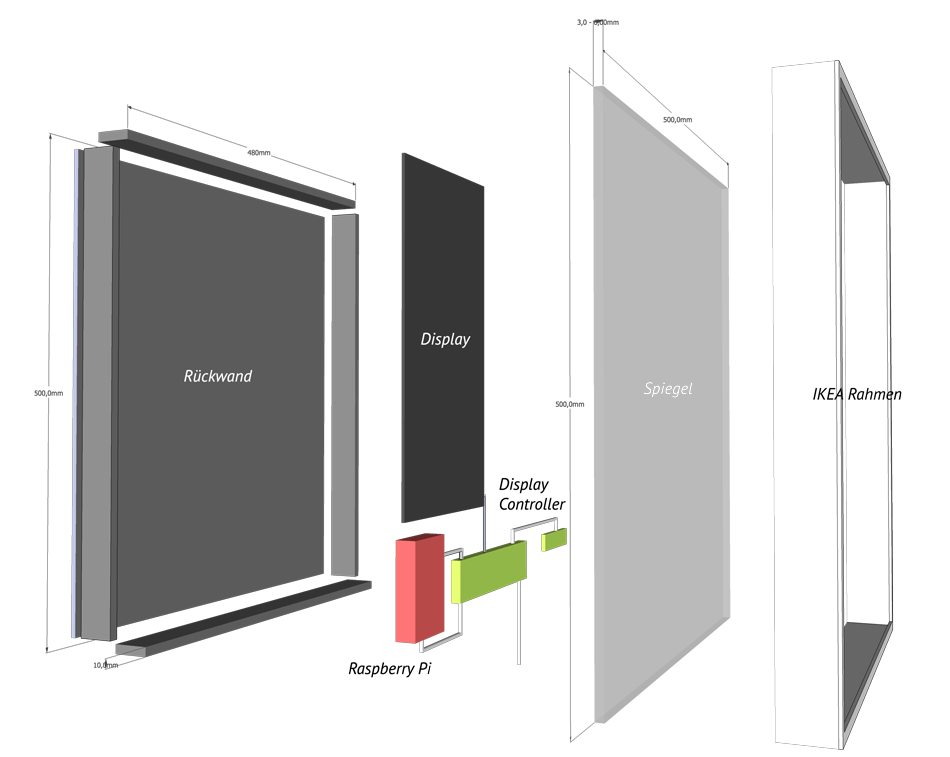
\includegraphics[scale=.5]{Bauteile.png} 
\caption{Hardware-Komponenten}
\end{figure}
\section{Raspberry Pi}
Der Raspberry Pi ist ein kompakter und günstiger aber vollwertiger Computer. Mit zahlreichen Schnittstellen und Modulen zur Erweiterung ist er sehr vielseitig einsetzbar und flexibel. In diesem Projekt wird ein Raspberry Pi 3 verwendet, das achte Modell der Reihe. Im Vergleich zu den Vorgängermodellen bringt dieser Raspberry Pi ein integriertes WLAN- und Bluetoothmodul mit. Zudem besitzt er 4 USB 2.0 Ports, einen HDMI-Anschluss, sowie einen analogen Video- und Audio-Ausgang. Sein Ethernet-Anschluss arbeitet mit 100 MBit/s. Der Prozessor nutzt vier ARMv8-Kerne. Aufgrund des verbauten Display- und Touch-Controllers kann der Raspberry Pi an ein LCD-Display oder einen Computermonitor angeschlossen werden. Über die GPIO-Leiste mit 26 GPIOs und insgesamt 40 Pins können weitere Module angesteuert werden oder Messaufgaben mit Sensoren übernommen werden. (Quelle: Heft c't Raspberry Pi Praxiswissen und Know-How für eigene Projekte S. 7 und S. 13)

Die Raspberry Pi Foundation entwickelt den Raspberry Pi und die dazugehörigen Module, wie die Kamera oder das LCD-Display. Das Ziel der Gründung ist das Vertreiben von kostengünstigen Produkten, mit welchen die Entwickler und Privatanwender die digitale Welt erschließen können und lernen mit jener umzugehen. Daher sind auf der Homepage des Raspberry Pis alle schematischen Zeichnungen der Modelle, sowie Dokumentationen bereitgestellt, die bei der Installation und der Programmentwicklung unterstützen. (www.raspberrypi.org)
Zudem weist die Foundation auf soziale Netzwerke und Foren, wie Github, hin und bietet Online-Training sowie Kurse an der Picadamie an.

The Raspberry Pi Foundation’s mission is to put the power of digital making into the hands of people all over the world. Our free training programmes form part of our strategy to achieve this challenging mission: we believe that everyone should have the opportunity to develop their computing and digital making skills.

Die Mission der Raspberry Pi Foundation ist es, die weitreichenden Möglichkeiten der Digitalisierung in die Hände der Menschen auf der ganzen Welt zu geben. Ein Teil dieser Strategie sind die kostenlosen Trainingsprogramme, die helfen, dieses wagemutige Mission zu erfüllen: Wir glauben jeder sollte die Möglichkeit haben, seine computertechnischen Fähigkeiten ausbauen zu können. (Zitat aus https://www.raspberrypi.org/training/)

\section{Sonstige Komponenten -> anderer Name}
Monitor VGA Adapter Spiegel für Prototyp
\chapter{Software}
\section{Betriebssystem}
\subsection*{Magic Mirror}
fra
\subsection*{MagicMirror\^2}
MagicMirror^1 ist eine open soure

\subsection*{Mirr.OS}
fa


Aufgrund der Vielzahl von Modulen und der breiten Communityabdeckung fiel die Entscheidung auf das MagicMirror hoch zwei Betriebssystem. 


Installation des Betriebssystem kann manuell oder automatisch durchgeführt werden. 
Für die automatische Installation kann folgender Befehl in der Konsole des Pis ausgeführt werden:
%\begin{lstlisting}
%https://raw.githubusercontent.com/MichMich/MagicMirror/master/installers/raspberry.sh

\section{Git}
Bei einem Project andem mehrere Personen beteiligt sind und man gleichzeitig einige Dokumente configuriert, modifiziert oder ersetzt können erhebliche kompatibilitätsprobleme entstehen. Um solche Probleme garnicht erst entstehen zu lassen wird in diesem Projekt das Programm GIT verwendet, welches es ermöglcht jeglichen Kontent auf dem neuesten Stand zu halten. Im wesentlichen ist Git eine freie Software zur verteilten Versionsverwaltung von Dateien und speichert die zu einem Projekt zugehörigen files in einem online-repository, welches sowohl lokal aber auch publik genutzt und geteilt werden kann. Aufgrund dieser Eigenschaften entstanden in den letzten Jahren dieverse Communities die gemeinsam an öffentlichen Projekten gearbeitet haben. Eines dieser Projekt ist der MagicMirror. Alle Module Readme-Dateien und Commits(fühere Versionen) eines Moduls stehen auf Github frei zur Verfügung und ermöglichen einen einfachen Einstieg in die Welt des MagicMirrors.

\subsection*{Der Einstieg in Git}
Um eigene Projekt anzulegen und dessen Inhalt mit bestimmten Personen zu Teilen oder zu bearbeiten ist es notwendig sich auf einem der vielen Git-Repository Anbietern online zu registrieren. Die Community des in unserem Fall verwendeten Betriebssystem Magicmirror^circle{2} nutzt ausschließlich Github, weshalb im weiteren Verlauf Git und Github als synonyme verwendet werden. 
\subsecion{Module}
Als Modul

Fabio


Die Dateien kommen alle aus der Github-Repository des Users MichMich. Dort können die Dateien auch manuell heruntergeladen und installiert werden. 
\section{Python und JavaScript}
Fa p fra j
\section{Konfiguration der Module}
\subsection{Fitbit}
\subsection{RSS Feeds}
\subsection{Google Kalender}
Fabio

dann noch meine eigenen Module
\section{badfg}






\chapter{Ergebnisse}
Screenshots von Bildschirm und fertiger Bildschirm
ich
\chapter{Ausblick}
ich
\end{document}